\chapter{Sprint 1 : Authentification et gestion des utilisateurs}


\newpage

\section{Introduction}

Le troisième chapitre présente les réalisations du Sprint 1. Nous détaillons les fonctionnalités liées à l’authentification, à la gestion des utilisateurs ainsi qu’à l’importation et l’extraction des données des factures.

\section{Backlog du Sprint}

\renewcommand{\arraystretch}{1.5}

\begin{table}[H]
	\centering
	\small
	\begin{tabularx}{\textwidth}{|c|p{3.8cm}|c|p{6cm}|c|}
		\hline
		\rowcolor{blue!20}
		\textbf{ID} & \textbf{User Story} & \textbf{ID-US} & \textbf{Tâche} & \textbf{Estimation} \\ \hline
		
		\multirow{4}{*}{1.1}
		& \multirow{4}{3.8cm}{En tant qu’utilisateur, je veux m’authentifier afin d’accéder au système.}
		& 1.1.1 & Conception des diagrammes UML. & \multirow{4}{*}{1 jour} \\ \cline{3-4}
		& & 1.1.2 & Développement de l’interface de connexion. & \\ \cline{3-4}
		& & 1.1.3 & Implémentation de l’API d’authentification. & \\ \cline{3-4}
		& & 1.1.4 & Tests et validation. & \\ \hline
		
		\multirow{4}{*}{1.2}
		& \multirow{4}{3.8cm}{En tant qu’administrateur, je veux gérer les utilisateurs afin de contrôler les accès.}
		& 1.2.1 & Conception UML de la gestion des utilisateurs. & \multirow{4}{*}{2 jours} \\ \cline{3-4}
		& & 1.2.2 & Développement des interfaces CRUD utilisateurs. & \\ \cline{3-4}
		& & 1.2.3 & Implémentation backend CRUD utilisateurs. & \\ \cline{3-4}
		& & 1.2.4 & Tests et validation. & \\ \hline
		
		\multirow{4}{*}{1.3}
		& \multirow{4}{3.8cm}{En tant que comptable, je veux importer une facture afin de lancer son traitement.}
		& 1.3.1 & Conception du processus d’importation. & \multirow{4}{*}{2 jours} \\ \cline{3-4}
		& & 1.3.2 & Développement de l’interface d’importation. & \\ \cline{3-4}
		& & 1.3.3 & Intégration de l’API d’importation. & \\ \cline{3-4}
		& & 1.3.4 & Tests d’importation. & \\ \hline
		
		\multirow{4}{*}{1.4}
		& \multirow{4}{3.8cm}{En tant que comptable, je veux extraire les données des factures via OCR/IA.}
		& 1.4.1 & Intégration du service OCR/IA. & \multirow{4}{*}{3 jours} \\ \cline{3-4}
		& & 1.4.2 & Traitement des données extraites. & \\ \cline{3-4}
		& & 1.4.3 & Stockage des résultats en base. & \\ \cline{3-4}
		& & 1.4.4 & Tests et validation. & \\ \hline
		
	\end{tabularx}
	\caption{Backlog détaillé du Sprint 1}
	\label{tab:backlog_sprint1}
\end{table}

\FloatBarrier

\section{Analyse}

\subsection{Analyse fonctionnelle}

\subsubsection{Diagramme de cas d’utilisation}

Le diagramme de cas d’utilisation montre clairement les fonctions principales du
premier sprint. Le diagramme de cas d’utilisation met en avant les interactions entre
les acteurs et le système, notamment l’authentification, la gestion des utilisateurs,
l’importation des factures et l’extraction des données.

\begin{figure}[H]
	\centering
	
\includegraphics[width=0.9\textwidth]{usecase_sprint1.jpg}
	\caption{Diagramme de cas d’utilisation du Sprint 1}
	\label{fig:usecase_sprint1}
\end{figure}
\subsubsection{Description textuelle des cas d’utilisation}

\subsubsection*{Cas d’utilisation : S’authentifier}

\begin{table}[H]
	\centering
	\renewcommand{\arraystretch}{1.35}
	\rowcolors{2}{gray!10}{white}
	
	\begin{tabularx}{\textwidth}{|p{2.8cm}|X|}
		\hline
		\rowcolor{blue!20}
		\textbf{Use Case} & S’authentifier \\ \hline
		
		\textbf{Acteur} & Utilisateur \\ \hline
		
		\textbf{Description} & Permet à l’utilisateur d’accéder au système de manière sécurisée à l’aide de ses identifiants. \\ \hline
		
		\textbf{Pré-condition} & La page de connexion est affichée. \\ \hline
		
		\rowcolor{blue!10}
		\textbf{Scénario nominal} &
		1- L’utilisateur entre l’adresse e-mail et le mot de passe. \newline
		2- Le système contrôle que les informations saisies sont valides. \newline
		3- Le système identifie le rôle de l’utilisateur. \newline
		4- Le système permet l’accès et envoie l’utilisateur à son interface principale. \\ \hline
		
		\textbf{Post-condition} & L’utilisateur est authentifié et accède à son espace. \\ \hline
		
		\rowcolor{blue!10}
		\textbf{Scénarios alternatifs} &
		1- Champs vides. \newline
		1.1- Le système montre un message d’erreur. \newline
		2- Les identifiants sont incorrects. \newline
		2.1- Le système refuse l’accès. \\ \hline
		
	\end{tabularx}
	
	\caption{Description textuelle du cas d’utilisation « S’authentifier »}
	\label{tab:authentification}
\end{table}



\subsubsection*{Cas d’utilisation : Gérer les utilisateurs}

\begin{table}[H]
	\centering
	\renewcommand{\arraystretch}{1.5}
	\small
	
	\begin{tabularx}{\textwidth}{|p{4.5cm}|X|}
		\hline
		\rowcolor{blue!20}
		\textbf{Nom du cas d’utilisation}
		& Gérer les utilisateurs \\ \hline
		
		\textbf{Description brève}
		& L’administrateur ajoute, modifie ou supprime les utilisateurs du système. \\ \hline
		
		\textbf{Acteurs primaires}
		& Administrateur \\ \hline
		
		\textbf{Acteurs secondaires}
		& Aucun \\ \hline
		
		\textbf{Pré-condition}
		& L’administrateur doit être authentifié. \\ \hline
		
		\textbf{Scénario nominal}
		&
		1- Le cas d’utilisation commence dès que l’administrateur ouvre l’interface de gestion des utilisateurs. \newline
		2- Le système affiche la liste des utilisateurs. Il indique les actions disponibles. \newline
		3- Si l’administrateur clique sur « Ajouter » : \newline
		\hspace*{0.5cm}3.1- Le système montre le formulaire d’ajout. \newline
		\hspace*{0.5cm}3.2- L’administrateur entre les données du nouvel utilisateur. \newline
		\hspace*{0.5cm}3.3- Le système contrôle les données saisies, le système garantit la cohérence. \newline
		\hspace*{0.5cm}3.4- Le système enregistre l’utilisateur. \newline
		\hspace*{0.5cm}3.5- Le système affiche un message de confirmation. \newline
		4- Si l’administrateur sélectionne « Modifier » : \newline
		\hspace*{0.5cm}4.1- Le système montre les informations de l’utilisateur sélectionné. \newline
		\hspace*{0.5cm}4.2- L’administrateur modifie les données voulues. \newline
		\hspace*{0.5cm}4.3- Le système enregistre les modifications. \newline
		\hspace*{0.5cm}4.4- Le système montre un message de confirmation. \newline
		5- Si l’administrateur sélectionne « Supprimer » : \newline
		\hspace*{0.5cm}5.1- Le système demande à l’utilisateur de confirmer. \newline
		\hspace*{0.5cm}5.2- L’administrateur confirme la suppression. \newline
		\hspace*{0.5cm}5.3- Le système supprime l’utilisateur. \newline
		\hspace*{0.5cm}5.4- Le système montre un message de confirmation. \\ \hline
		
		\textbf{Post-condition}
		& Les informations des utilisateurs sont mises à jour dans le système. \\ \hline
		
		\textbf{Scénarios alternatifs}
		&
		1- Informations invalides ou incomplètes. \newline
		1.1- Le système affiche un message d’erreur. \newline
		2- Adresse email déjà utilisée. \newline
		2.1- Le système refuse l’enregistrement. \newline
		3- Utilisateur introuvable. \newline
		3.1- Le système annule l’opération. \\ \hline
		
	\end{tabularx}
	
	\caption{Description textuelle du cas d’utilisation « Gérer les utilisateurs »}
	\label{tab:gerer_utilisateurs}
\end{table}

\FloatBarrier

\subsection{Analyse dynamique}

\subsubsection{Diagramme de séquence système du cas d’utilisation « S’authentifier »}

Le diagramme de séquence du système montre les échanges entre l’utilisateur et le système pendant l’authentification. Le diagramme décrit le déroulement de l’authentification.

\begin{figure}[H]
	\centering
	
\includegraphics[width=0.85\textwidth]{seq_auth.jpg}
	\caption{Diagramme de séquence système du cas d’utilisation « S’authentifier »}
	\label{fig:seq_auth}
\end{figure}

\FloatBarrier

\subsubsection{Diagramme de séquence système du cas d’utilisation « Gérer les utilisateurs »}

Le diagramme de séquence du système montre comment l’administrateur interagit avec le système lors de la gestion des utilisateurs.

\begin{figure}[H]
	\centering
	
\includegraphics[width=0.85\textwidth]{seq_manage_users.jpg}
	\caption{Diagramme de séquence système du cas d’utilisation « Gérer les utilisateurs »}
	\label{fig:seq_manage_users}
\end{figure}

\FloatBarrier

\section{Conception}
\subsection{Conception statique}

\subsubsection{Diagramme de classes du Sprint 1}

Je constate que le diagramme de classes montre la structure du système pendant le premier sprint. Le diagramme de classes met en avant les classes principales : l’utilisateur, l’administrateur, le rôle et la facture.

\begin{figure}[H]
	\centering
	
\includegraphics[width=0.85\textwidth]{diagramme_classe.jpg}
	\caption{Diagramme de classes du Sprint 1}
	\label{fig:class_sprint1}
\end{figure}

\FloatBarrier
\subsection{Conception dynamique}

\subsubsection{Diagramme de séquence détaillé du cas d’utilisation « S’authentifier »}

Le diagramme de séquence détaillé suivant illustre les interactions entre l’interface d’authentification, le contrôleur, le service utilisateur et la base de données lors du processus d’authentification.

\begin{figure}[H]
	\centering
	
\includegraphics[width=0.85\textwidth]{seq_auth_detail.jpg}
	\caption{Diagramme de séquence détaillé du cas d’utilisation « S’authentifier »}
	\label{fig:seq_auth_detail}
\end{figure}

\FloatBarrier

\subsubsection{Diagramme de séquence détaillé du cas d’utilisation « Gérer les utilisateurs »}

Le diagramme de séquence ci-dessous montre comment l’administrateur, l’interface de gestion des utilisateurs, le contrôleur, le service utilisateur et la base de données interagissent pendant la gestion des comptes.

\begin{figure}[H]
	\centering
	
\includegraphics[width=0.85\textwidth]{seq_manage_users_detail.jpg}
	\caption{Diagramme de séquence détaillé du cas d’utilisation « Gérer les utilisateurs »}
	\label{fig:seq_manage_users_detail}
\end{figure}

\FloatBarrier


\section{Implémentation}

\subsection{Dictionnaire de données}

\subsubsection{Table utilisateur}

\renewcommand{\arraystretch}{1.3}

\begin{table}[H]
	\centering
	\footnotesize
	
	\begin{tabularx}{\textwidth}{|p{3cm}|p{2.5cm}|p{3.5cm}|X|}
		\hline
		
		\rowcolor{blue!20}
		\textbf{Nom du champ}
		&
		\textbf{Type}
		&
		\textbf{Contraintes}
		&
		\textbf{Description}
		\\ \hline
		
		id\_utilisateur
		&
		BIGINT
		&
		PRIMARY KEY
		&
		Identifiant unique de l’utilisateur.
		\\ \hline
		
		nom
		&
		VARCHAR
		&
		NOT NULL
		&
		Nom complet de l’utilisateur.
		\\ \hline
		
		email
		&
		VARCHAR
		&
		UNIQUE, NOT NULL
		&
		Adresse email utilisée pour l’authentification.
		\\ \hline
		
		motdepasse
		&
		VARCHAR
		&
		NOT NULL
		&
		Mot de passe chiffré de l’utilisateur.
		\\ \hline
		
		role
		&
		VARCHAR
		&
		NOT NULL
		&
		Rôle attribué à l’utilisateur.
		\\ \hline
		
	\end{tabularx}
	
	\caption{Dictionnaire de données de la table utilisateur}
	\label{tab:user_table}
	
\end{table}



\subsubsection{Table importation}

\begin{table}[H]
	\centering
	\footnotesize
	
	\begin{tabularx}{\textwidth}{|p{3cm}|p{2.5cm}|p{3.5cm}|X|}
		\hline
		
		\rowcolor{blue!20}
		\textbf{Nom du champ}
		&
		\textbf{Type}
		&
		\textbf{Contraintes}
		&
		\textbf{Description}
		\\ \hline
		
		id\_import
		&
		BIGINT
		&
		PRIMARY KEY
		&
		Identifiant unique de l’importation.
		\\ \hline
		
		nomFichier
		&
		VARCHAR
		&
		NOT NULL
		&
		Nom du fichier importé.
		\\ \hline
		
		dateImport
		&
		DATETIME
		&
		NOT NULL
		&
		Date d’importation du fichier.
		\\ \hline
		
		utilisateur
		&
		BIGINT
		&
		FOREIGN KEY
		&
		Utilisateur ayant effectué l’importation.
		\\ \hline
		
		statut
		&
		VARCHAR
		&
		NOT NULL
		&
		État de traitement du fichier.
		\\ \hline
		
	\end{tabularx}
	
	\caption{Dictionnaire de données de la table importation}
	\label{tab:import_table}
	
\end{table}
\section{Réalisation}

\subsection{Interfaces utilisateur}

\subsubsection{Interface de connexion}

L’interface de connexion donne à l’utilisateur un accès sécurisé au système. L’interface de connexion comprend les champs pour saisir l’adresse email et le mot de passe. Le système valide les informations saisies. Le système redirige l’utilisateur vers son espace selon le rôle de l’utilisateur.

\begin{figure}[H]
	\centering
	
\includegraphics[width=0.4\textwidth]{login.jpg}
	\caption{Interface de connexion du système}
	\label{fig:login}
\end{figure}

\FloatBarrier

\subsubsection{Interface de liste des utilisateurs}

Cette interface permet à l’administrateur de voir la liste des utilisateurs du système. L’administrateur peut aussi ajouter, modifier ou supprimer un compte utilisateur.

\begin{figure}[H]
	\centering
	
\includegraphics[width=0.65\textwidth]{users_list.jpg}
	\caption{Interface de liste des utilisateurs}
	\label{fig:users_list}
\end{figure}

\FloatBarrier

\subsubsection{Interface d’ajout d’un utilisateur}

L’administrateur utilise l’interface pour créer un nouveau compte utilisateur. L’interface comprend les champs nécessaires : le nom, l’adresse email, le mot de passe et le rôle de l’utilisateur.

\begin{figure}[H]
	\centering
	
\includegraphics[width=0.65\textwidth]{add_user.jpg}
	\caption{Interface d’ajout d’un utilisateur}
	\label{fig:add_user}
\end{figure}

\FloatBarrier

\subsubsection{Interface de modification d’un utilisateur}

L’administrateur modifie les informations d’un utilisateur existant grâce à l’interface. L’interface propose des champs déjà remplis pour simplifier la mise à jour des données avant la validation.

\begin{figure}[H]
	\centering
	
\includegraphics[width=0.75\textwidth]{edit_user.jpg}
	\caption{Interface de modification d’un utilisateur}
	\label{fig:edit_user}
\end{figure}

\FloatBarrier

\subsubsection{Interface d’importation des factures}

L’interface permet au comptable d’importer une facture dans le système. Après la sélection du fichier, le traitement démarre pour préparer l’extraction automatique des données.

\begin{figure}[H]
	\centering
	
\includegraphics[width=0.75\textwidth]{ui_import.jpg}
	\caption{Interface d’importation des factures}
	\label{fig:ui_import}
\end{figure}

\FloatBarrier

\subsubsection{Interface d’affichage des résultats OCR}

Cette interface permet au comptable de consulter les données extraites automatiquement à partir de la facture importée. L’interface montre les informations principales : le fournisseur, la date, les montants et le numéro de facture.

\begin{figure}[H]
	\centering
	
\includegraphics[width=0.75\textwidth]{ui_ocr_result.jpg}
	\caption{Interface d’affichage des résultats OCR}
	\label{fig:ui_ocr_result}
\end{figure}
\section{Tests Postman}

Cette section présente les tests réalisés avec l’outil Postman afin de vérifier le bon fonctionnement des API développées durant le Sprint 1.  
Ces tests concernent principalement l’authentification des utilisateurs, la gestion des comptes ainsi que les opérations de base liées aux utilisateurs.

L’objectif de ces tests est de s’assurer que chaque requête envoyée au backend retourne une réponse correcte et que les données sont bien traitées par le système.

\renewcommand{\arraystretch}{1.5}

\begin{longtable}{|>{\centering\arraybackslash}m{6cm}|>{\centering\arraybackslash}m{10cm}|}
	\hline
	
	\rowcolor{blue!20}
	\textbf{Description} & \textbf{Capture}
	\\ \hline
	
	Cette requête permet à l’utilisateur de se connecter à la plateforme en utilisant son adresse email et son mot de passe. 
	Elle permet de vérifier l’API d’authentification ainsi que la redirection de l’utilisateur selon son rôle.
	&
	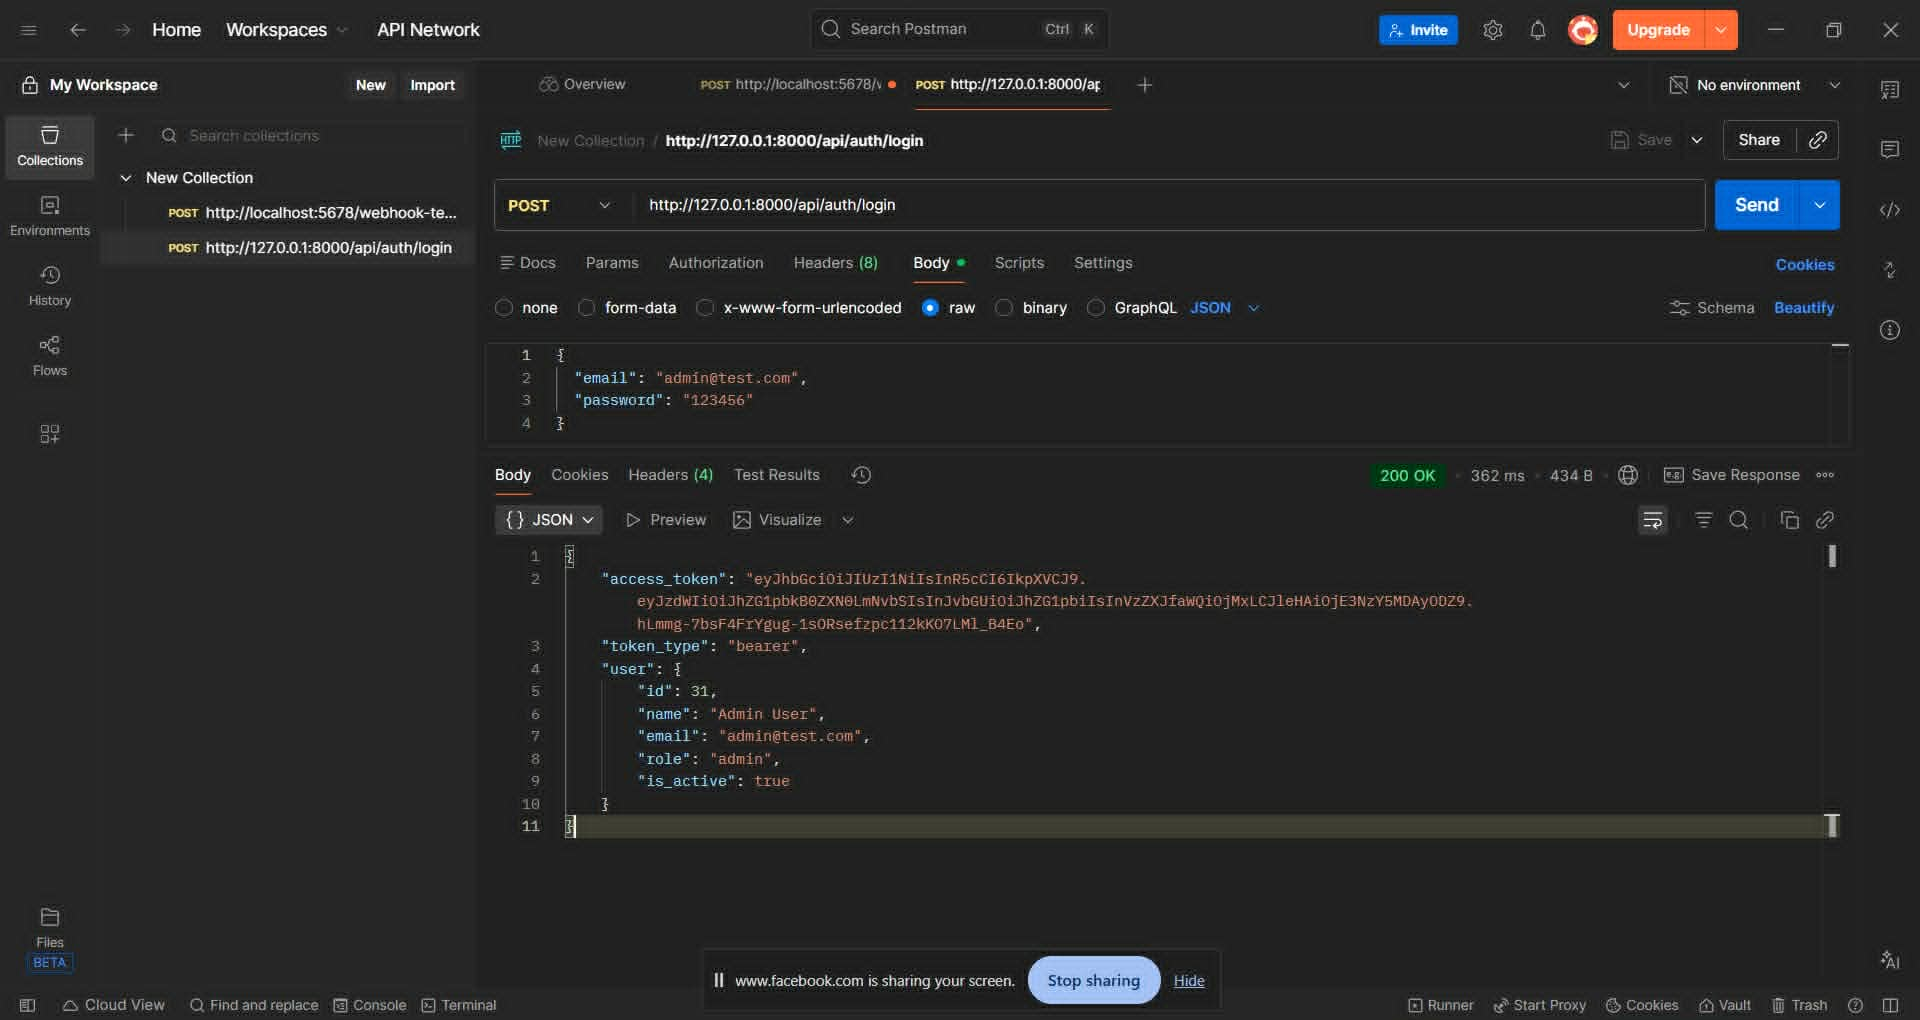
\includegraphics[width=8cm]{figures/postman_login.jpg}
	\\ \hline
	
	Cette requête permet à l’administrateur d’ajouter un nouvel utilisateur dans le système. 
	Elle vérifie l’enregistrement des informations saisies telles que le nom, l’email, le mot de passe et le rôle.
	&
	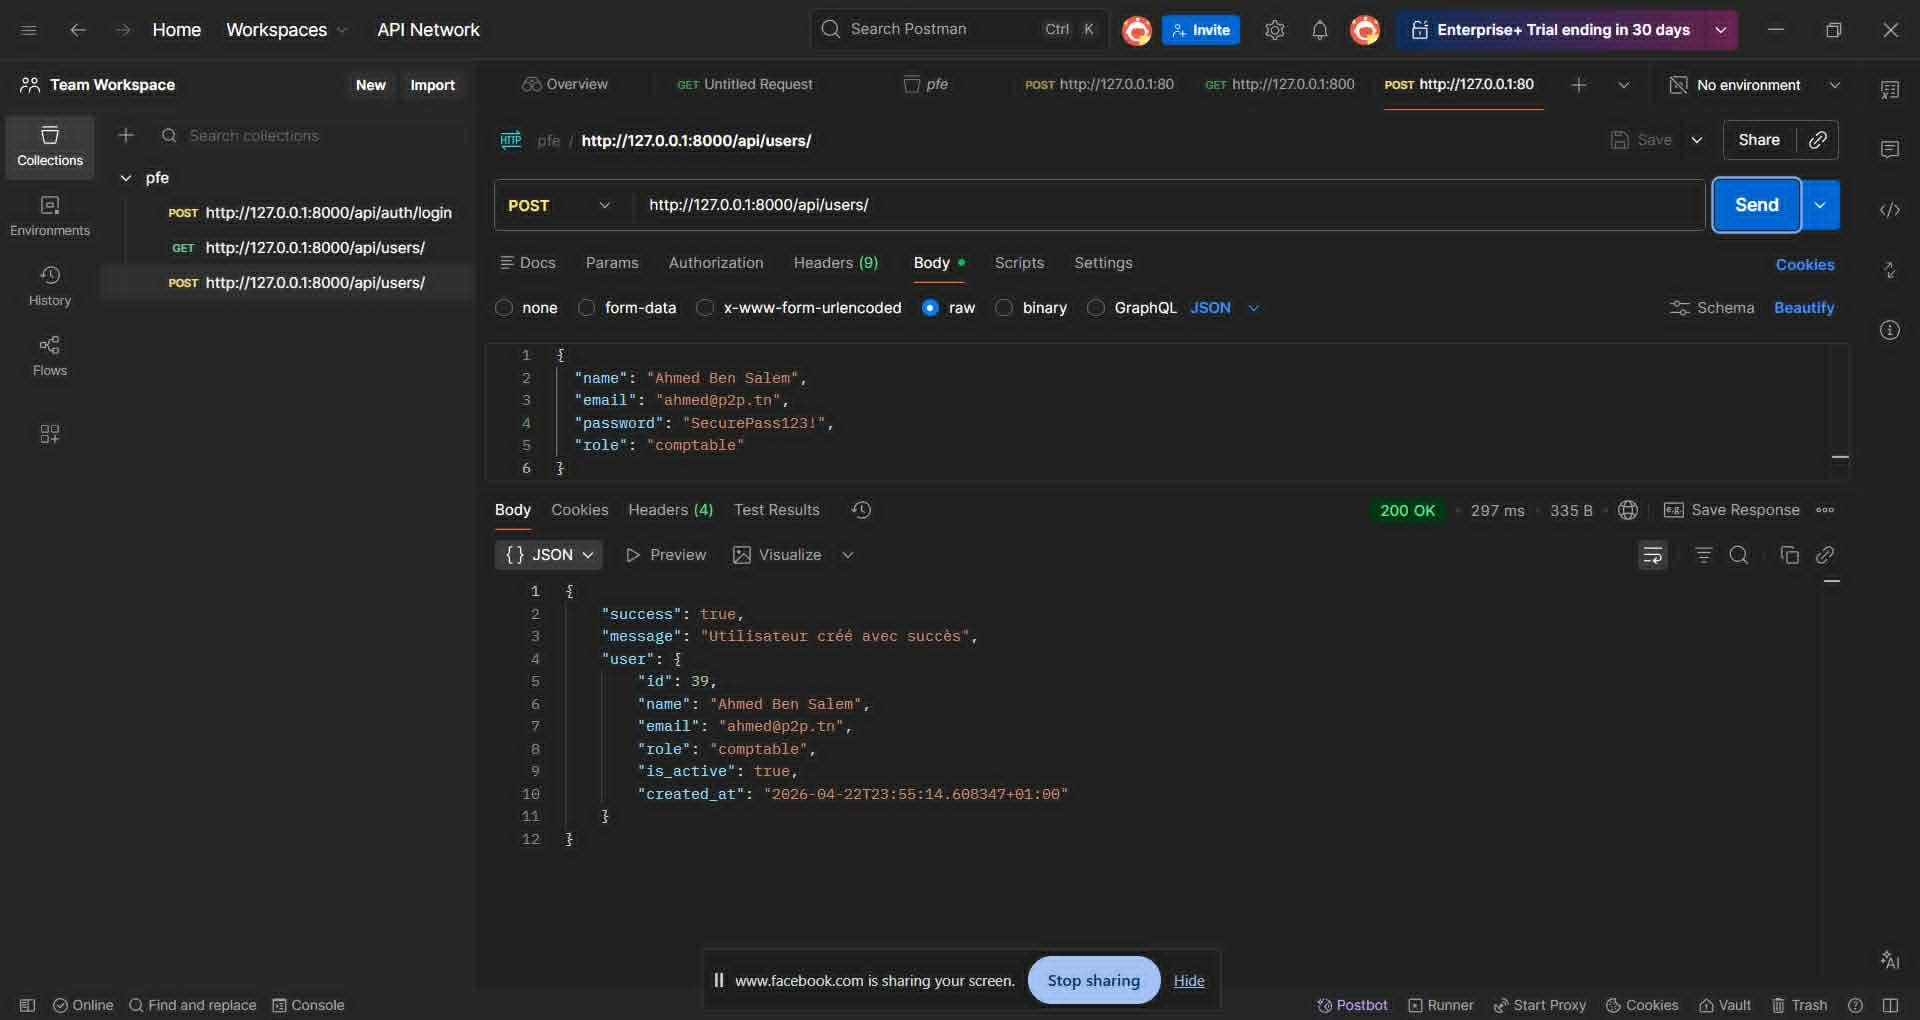
\includegraphics[width=8cm]{figures/postman_add_user.jpg}
	\\ \hline
	
	Cette requête permet de modifier les informations d’un utilisateur existant. 
	Elle permet de tester la mise à jour des données dans la base et de vérifier que les changements sont bien sauvegardés.
	&
	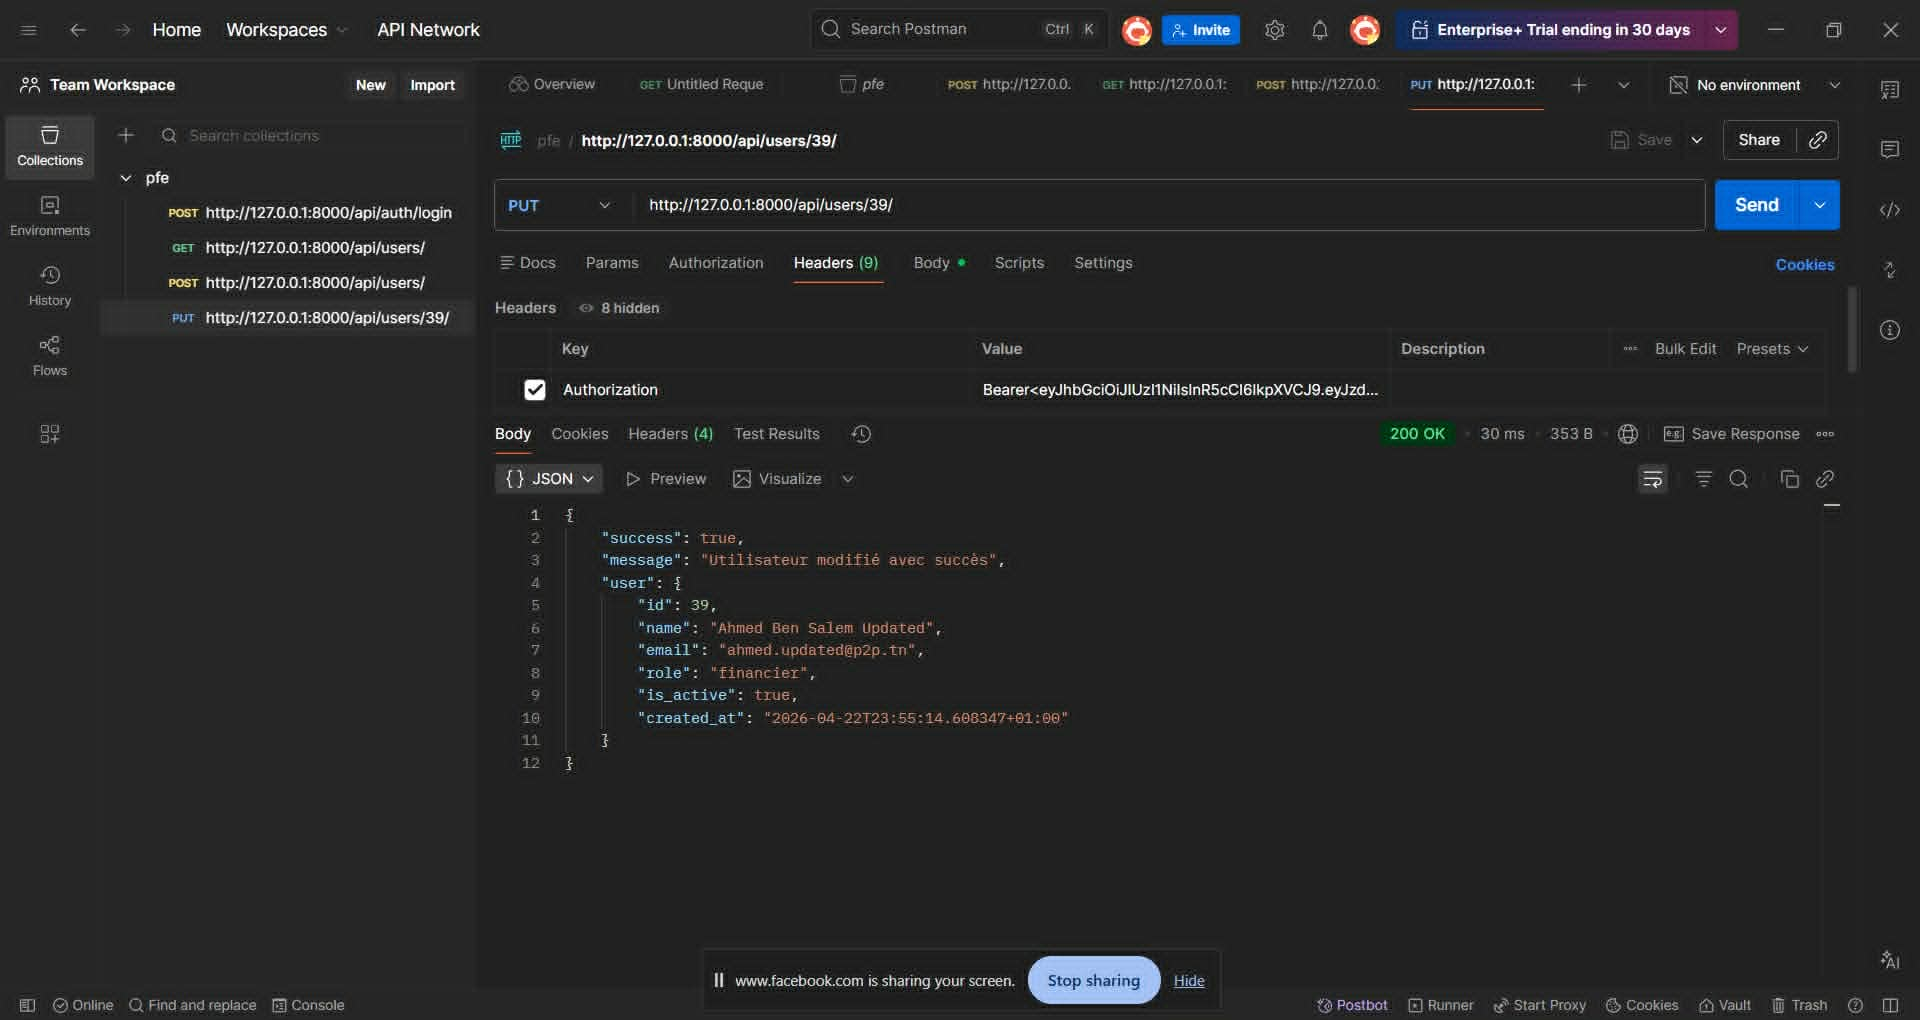
\includegraphics[width=8cm]{figures/postman_update_user.jpg}
	\\ \hline
	
	Cette requête permet de supprimer un utilisateur du système. 
	Elle vérifie que l’utilisateur sélectionné est bien supprimé de la base de données.
	&
	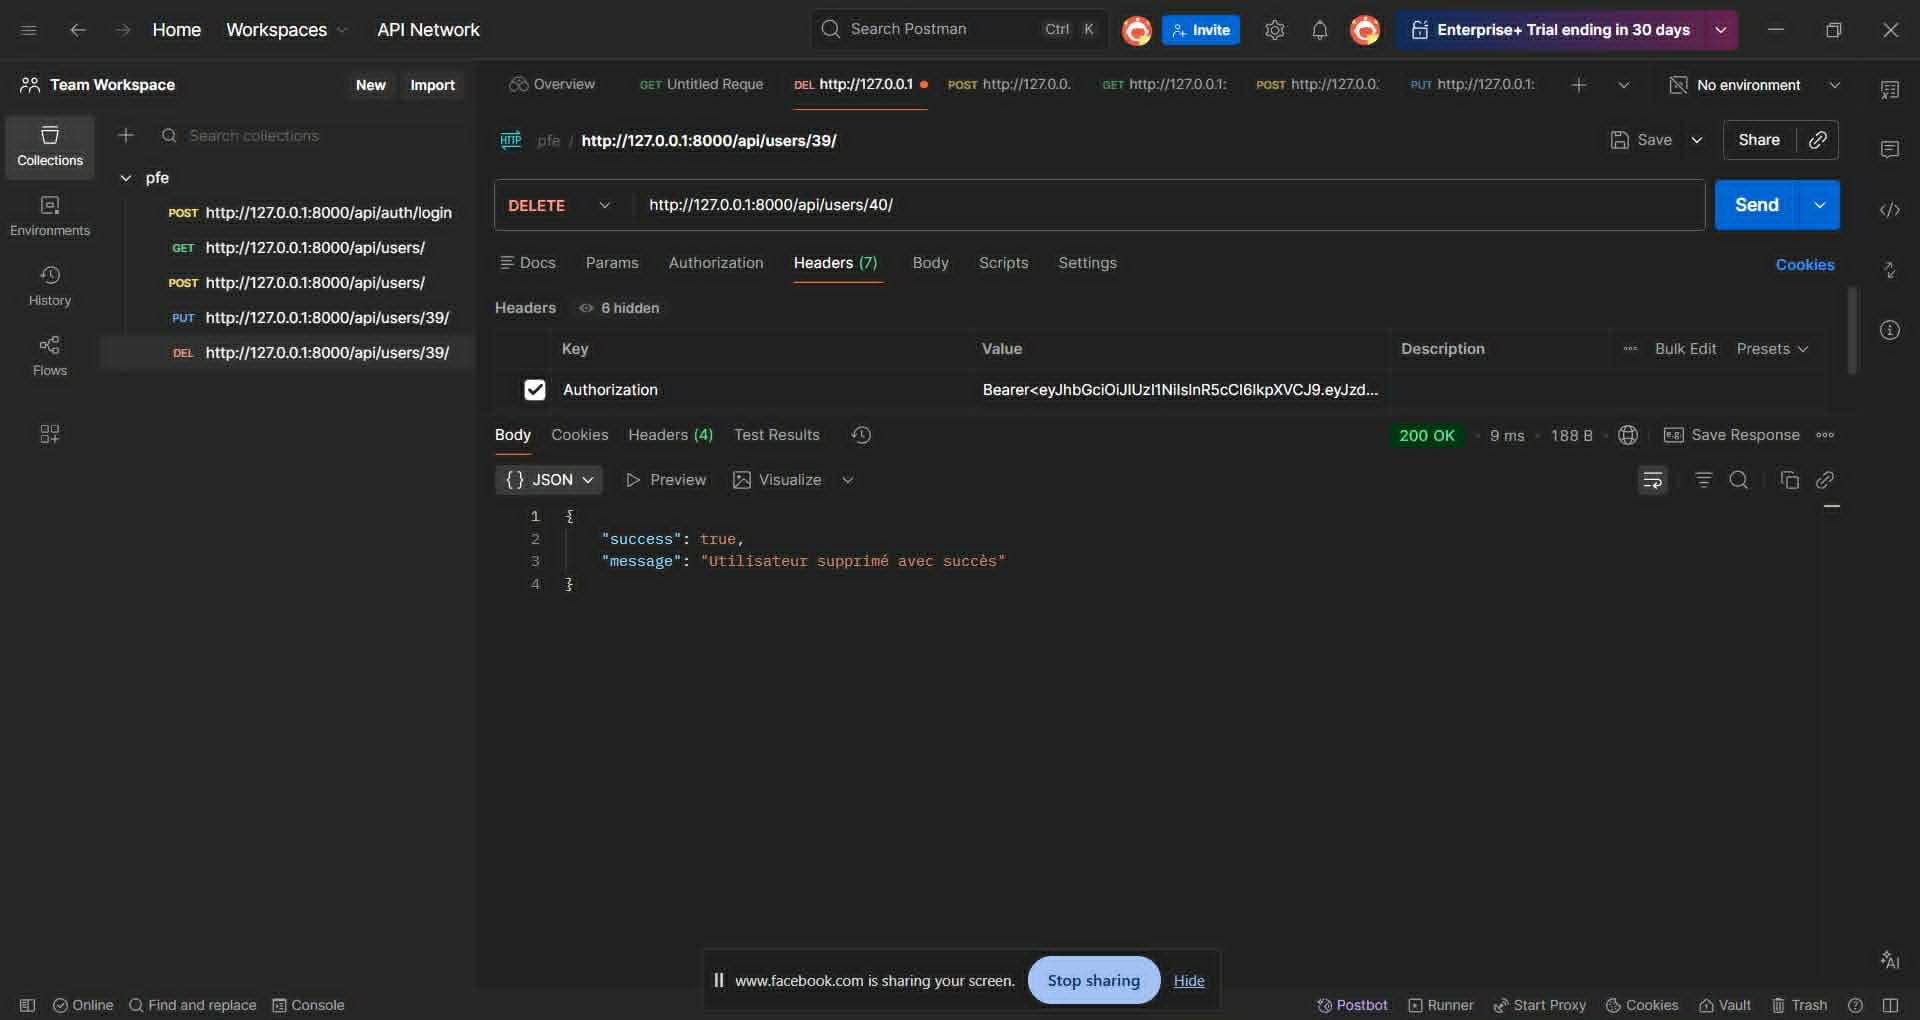
\includegraphics[width=8cm]{figures/postman_delete_user.jpg}
	\\ \hline
	
	Cette requête permet de récupérer la liste des utilisateurs enregistrés dans le système. 
	Elle sert à vérifier l’affichage des comptes existants et le bon fonctionnement de l’API de consultation.
	&
	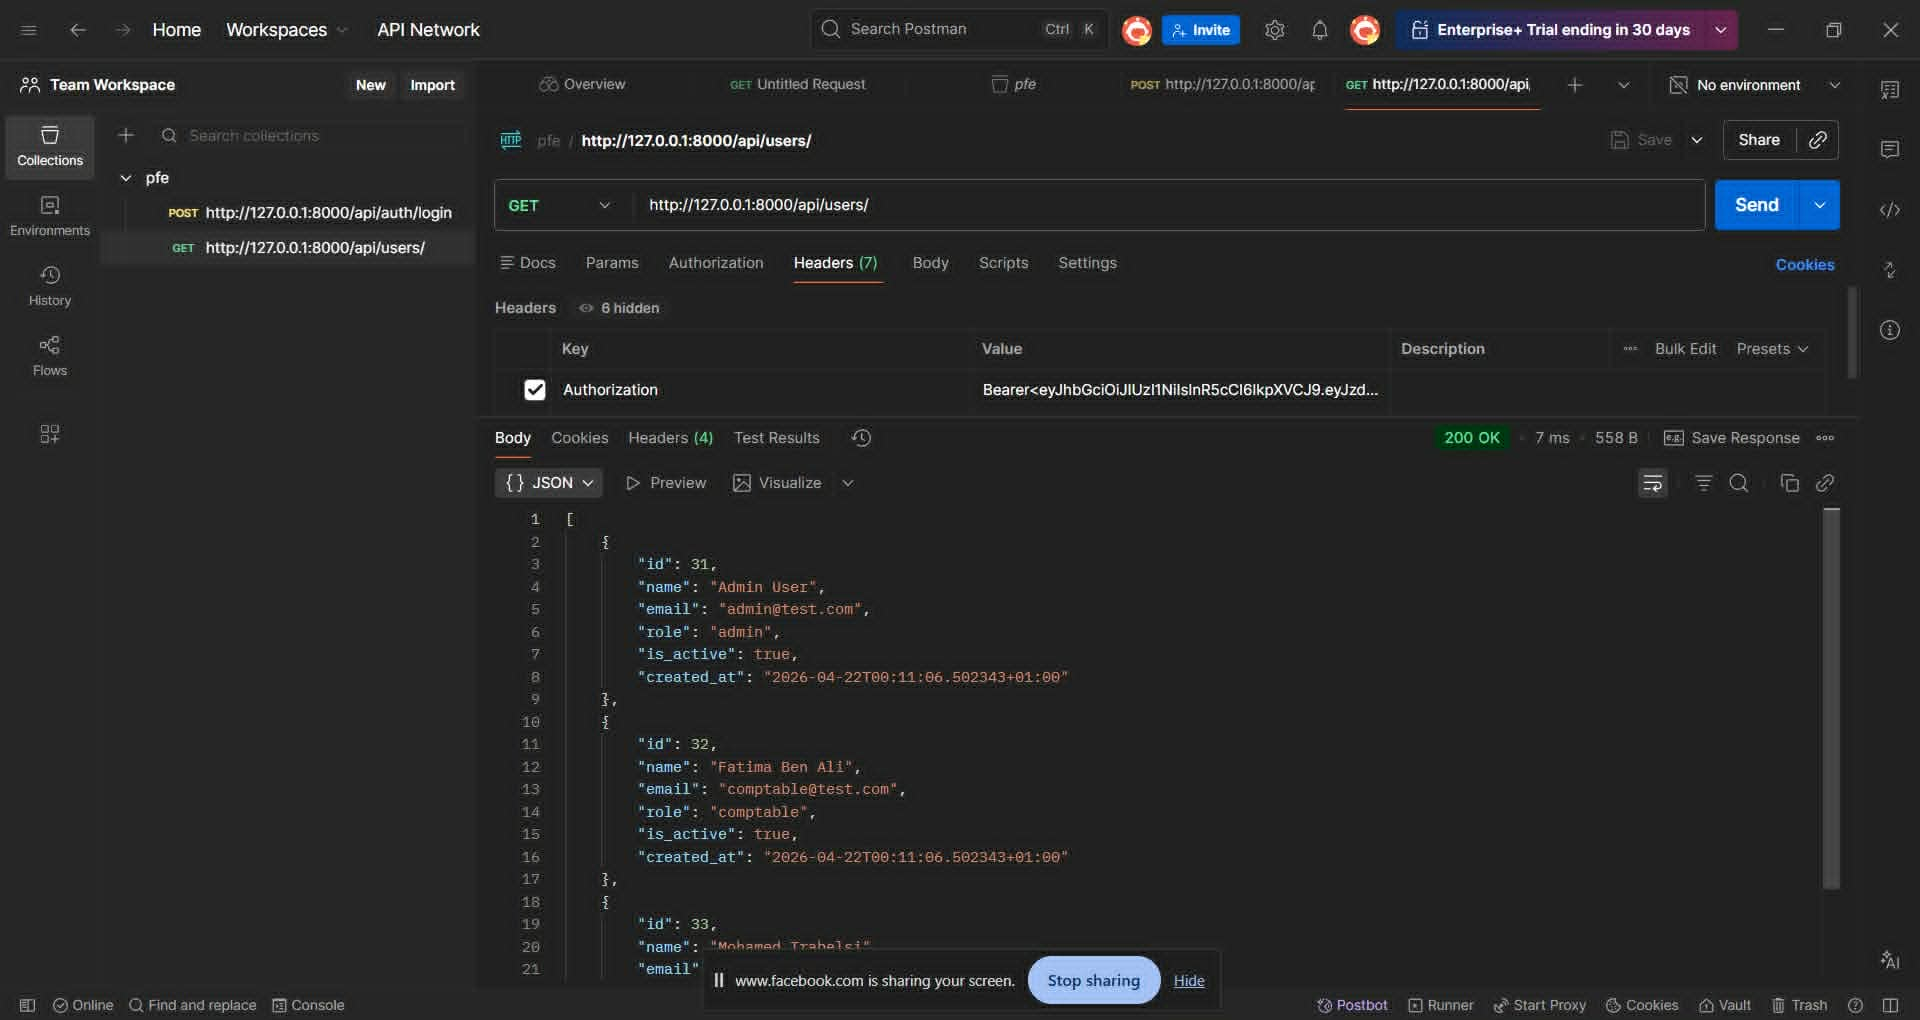
\includegraphics[width=8cm]{figures/postman_users.jpg}
	\\ \hline
	
	\caption{Tests Postman du Sprint 1}
\end{longtable}
\vspace{-0.2cm}
\subsection{Revue de Sprint}

La revue du Sprint 1 a permis de présenter les fonctionnalités réalisées liées à
l’authentification, à la gestion des utilisateurs ainsi qu’à l’importation et à
l’extraction des factures via OCR et intelligence artificielle. Cette étape a permis
de vérifier le bon fonctionnement des interfaces développées, des API
d’authentification ainsi que des mécanismes d’importation et de traitement des données.

\vspace{-0.2cm}
\noindent\textbf{Burndown Chart :} Le Burndown Chart du Sprint 1 permet de visualiser
l’évolution du travail restant durant les fonctionnalités d’authentification, de gestion
des utilisateurs et d’extraction des données. Le graphique montre une progression
régulière des tâches jusqu’à la finalisation du sprint. Comme présenté dans la figure
\ref{fig:brun1}.

\vspace{-0.4cm}
\begin{figure}[H]
	\centering
	
\includegraphics[width=0.5\textwidth]{burndown_sprint1.jpg}
	\caption{Diagramme de Burndown Chart du Sprint 1}
	\label{fig:brun1}
\end{figure}
\begin{table}[H]
	\centering
	\renewcommand{\arraystretch}{1.3}
	
	\begin{tabular}{|c|p{5cm}|c|}
		\hline
		\rowcolor{blue!20}
		\textbf{ID User Story} & \textbf{Fonctionnalité} & \textbf{Estimation} \\
		\hline
		
		1.1 & Authentification des utilisateurs & 3 \\
		\hline
		
		1.2 & Gestion des utilisateurs & 3 \\
		\hline
		
		1.3 & Importation des factures & 4 \\
		\hline
		
		1.4 & Extraction OCR des données & 5 \\
		\hline
		
		1.5 & Tests Postman des API & 2 \\
		\hline
		
		1.6 & Intégration Frontend / Backend & 3 \\
		\hline
		
		\multicolumn{2}{|c|}{\textbf{Vélocité totale estimée}} & \textbf{20} \\
		\hline
		
	\end{tabular}
	
	\caption{Calcul de vélocité estimée du Sprint 1}
\end{table}
\section{Conclusion}

Dans ce chapitre, nous avons présenté les fonctionnalités développées durant le Sprint 1. Nous avons réalisé l’authentification, la gestion des utilisateurs ainsi que l’importation et l’extraction automatique des données des factures.